% Created by tikzDevice version 0.6.2 on 2014-03-28 11:37:47
% !TEX encoding = UTF-8 Unicode
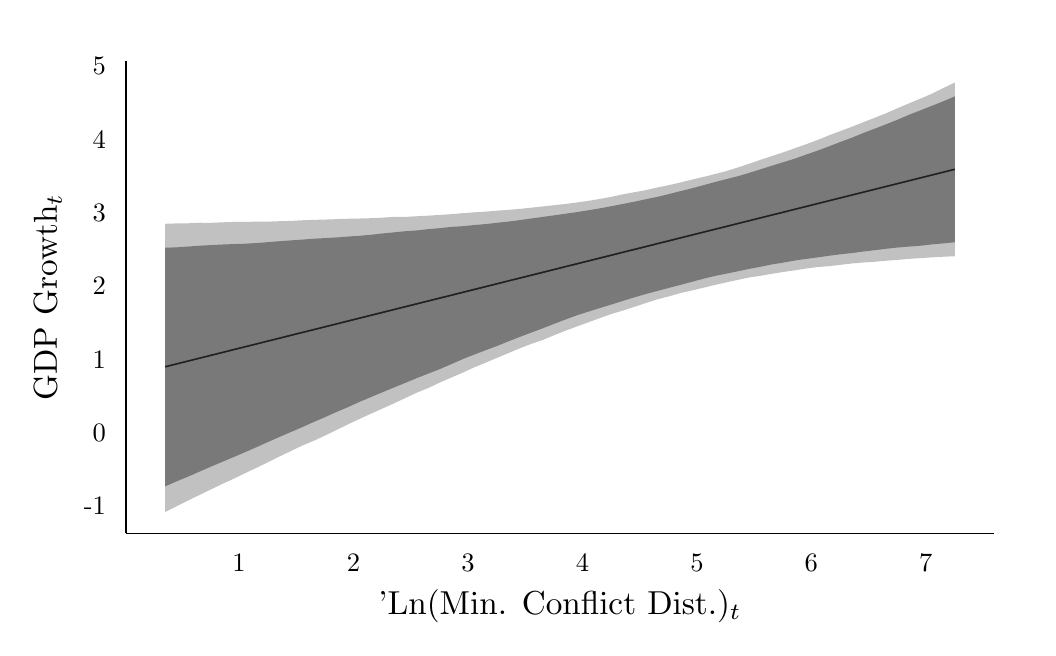
\begin{tikzpicture}[x=1pt,y=1pt]
\definecolor[named]{drawColor}{rgb}{0.00,0.00,0.00}
\definecolor[named]{fillColor}{rgb}{1.00,1.00,1.00}
\fill[color=fillColor,fill opacity=0.00,] (0,0) rectangle (361.35,216.81);
\begin{scope}
\path[clip] (  0.00,  0.00) rectangle (361.35,216.81);
\end{scope}
\begin{scope}
\path[clip] (  0.00,  0.00) rectangle (361.35,216.81);
\end{scope}
\begin{scope}
\path[clip] (  0.00,  0.00) rectangle (361.35,216.81);
\definecolor[named]{drawColor}{rgb}{1.00,1.00,1.00}
\definecolor[named]{fillColor}{rgb}{1.00,1.00,1.00}

\draw[color=drawColor,line width= 0.6pt,line cap=round,line join=round,fill=fillColor,] ( -0.00,  0.00) rectangle (361.35,216.81);
\end{scope}
\begin{scope}
\path[clip] (  0.00,  0.00) rectangle (361.35,216.81);
\end{scope}
\begin{scope}
\path[clip] (  0.00,  0.00) rectangle (361.35,216.81);
\end{scope}
\begin{scope}
\path[clip] (  0.00,  0.00) rectangle (361.35,216.81);
\end{scope}
\begin{scope}
\path[clip] ( 35.42, 34.03) rectangle (349.30,204.77);
\definecolor[named]{fillColor}{rgb}{1.00,1.00,1.00}

\draw[fill=fillColor,draw opacity=0.00,] ( 35.42, 34.03) rectangle (349.31,204.77);
\definecolor[named]{drawColor}{rgb}{0.00,0.00,0.00}
\definecolor[named]{fillColor}{rgb}{0.00,0.00,0.00}

\draw[color=drawColor,line width= 0.6pt,line join=round,] ( 49.69, 94.28) --
	( 53.82, 95.31) --
	( 57.96, 96.35) --
	( 62.09, 97.38) --
	( 66.23, 98.42) --
	( 70.37, 99.45) --
	( 74.50,100.49) --
	( 78.64,101.52) --
	( 82.77,102.55) --
	( 86.91,103.59) --
	( 91.04,104.62) --
	( 95.18,105.66) --
	( 99.31,106.69) --
	(103.45,107.72) --
	(107.59,108.76) --
	(111.72,109.79) --
	(115.86,110.83) --
	(119.99,111.86) --
	(124.13,112.90) --
	(128.26,113.93) --
	(132.40,114.96) --
	(136.53,116.00) --
	(140.67,117.03) --
	(144.80,118.07) --
	(148.94,119.10) --
	(153.08,120.13) --
	(157.21,121.17) --
	(161.35,122.20) --
	(165.48,123.24) --
	(169.62,124.27) --
	(173.75,125.31) --
	(177.89,126.34) --
	(182.02,127.37) --
	(186.16,128.41) --
	(190.30,129.44) --
	(194.43,130.48) --
	(198.57,131.51) --
	(202.70,132.54) --
	(206.84,133.58) --
	(210.97,134.61) --
	(215.11,135.65) --
	(219.24,136.68) --
	(223.38,137.71) --
	(227.51,138.75) --
	(231.65,139.78) --
	(235.79,140.82) --
	(239.92,141.85) --
	(244.06,142.89) --
	(248.19,143.92) --
	(252.33,144.95) --
	(256.46,145.99) --
	(260.60,147.02) --
	(264.73,148.06) --
	(268.87,149.09) --
	(273.01,150.12) --
	(277.14,151.16) --
	(281.28,152.19) --
	(285.41,153.23) --
	(289.55,154.26) --
	(293.68,155.30) --
	(297.82,156.33) --
	(301.95,157.36) --
	(306.09,158.40) --
	(310.22,159.43) --
	(314.36,160.47) --
	(318.50,161.50) --
	(322.63,162.53) --
	(326.77,163.57) --
	(330.90,164.60) --
	(335.04,165.64);
\definecolor[named]{fillColor}{rgb}{0.20,0.20,0.20}

\draw[fill=fillColor,fill opacity=0.30,draw opacity=0.00,] ( 49.69,145.94) --
	( 53.82,146.07) --
	( 57.96,146.12) --
	( 62.09,146.32) --
	( 66.23,146.30) --
	( 70.37,146.47) --
	( 74.50,146.61) --
	( 78.64,146.60) --
	( 82.77,146.74) --
	( 86.91,146.73) --
	( 91.04,146.87) --
	( 95.18,146.98) --
	( 99.31,147.22) --
	(103.45,147.36) --
	(107.59,147.47) --
	(111.72,147.61) --
	(115.86,147.77) --
	(119.99,147.85) --
	(124.13,147.96) --
	(128.26,148.16) --
	(132.40,148.45) --
	(136.53,148.43) --
	(140.67,148.67) --
	(144.80,148.88) --
	(148.94,149.15) --
	(153.08,149.41) --
	(157.21,149.77) --
	(161.35,150.07) --
	(165.48,150.33) --
	(169.62,150.68) --
	(173.75,150.98) --
	(177.89,151.33) --
	(182.02,151.76) --
	(186.16,152.21) --
	(190.30,152.67) --
	(194.43,153.11) --
	(198.57,153.65) --
	(202.70,154.25) --
	(206.84,154.92) --
	(210.97,155.69) --
	(215.11,156.59) --
	(219.24,157.35) --
	(223.38,158.09) --
	(227.51,159.04) --
	(231.65,159.90) --
	(235.79,160.84) --
	(239.92,161.87) --
	(244.06,162.83) --
	(248.19,163.87) --
	(252.33,164.94) --
	(256.46,166.23) --
	(260.60,167.59) --
	(264.73,169.03) --
	(268.87,170.39) --
	(273.01,171.75) --
	(277.14,173.21) --
	(281.28,174.67) --
	(285.41,176.21) --
	(289.55,177.89) --
	(293.68,179.44) --
	(297.82,180.99) --
	(301.95,182.63) --
	(306.09,184.25) --
	(310.22,185.88) --
	(314.36,187.72) --
	(318.50,189.46) --
	(322.63,191.17) --
	(326.77,192.94) --
	(330.90,195.01) --
	(335.04,197.00) --
	(335.04,134.22) --
	(330.90,134.04) --
	(326.77,133.81) --
	(322.63,133.53) --
	(318.50,133.27) --
	(314.36,132.90) --
	(310.22,132.60) --
	(306.09,132.21) --
	(301.95,131.95) --
	(297.82,131.60) --
	(293.68,131.11) --
	(289.55,130.63) --
	(285.41,130.31) --
	(281.28,129.78) --
	(277.14,129.12) --
	(273.01,128.53) --
	(268.87,127.87) --
	(264.73,127.14) --
	(260.60,126.54) --
	(256.46,125.64) --
	(252.33,124.75) --
	(248.19,123.82) --
	(244.06,122.81) --
	(239.92,121.81) --
	(235.79,120.90) --
	(231.65,119.70) --
	(227.51,118.64) --
	(223.38,117.32) --
	(219.24,115.95) --
	(215.11,114.60) --
	(210.97,113.37) --
	(206.84,111.90) --
	(202.70,110.38) --
	(198.57,108.87) --
	(194.43,107.35) --
	(190.30,105.70) --
	(186.16,103.98) --
	(182.02,102.57) --
	(177.89,100.98) --
	(173.75, 99.24) --
	(169.62, 97.51) --
	(165.48, 95.74) --
	(161.35, 94.06) --
	(157.21, 92.17) --
	(153.08, 90.38) --
	(148.94, 88.60) --
	(144.80, 86.62) --
	(140.67, 84.95) --
	(136.53, 83.01) --
	(132.40, 81.05) --
	(128.26, 79.21) --
	(124.13, 77.38) --
	(119.99, 75.45) --
	(115.86, 73.55) --
	(111.72, 71.50) --
	(107.59, 69.49) --
	(103.45, 67.56) --
	( 99.31, 65.84) --
	( 95.18, 63.88) --
	( 91.04, 61.88) --
	( 86.91, 59.82) --
	( 82.77, 57.83) --
	( 78.64, 55.86) --
	( 74.50, 53.85) --
	( 70.37, 51.96) --
	( 66.23, 49.97) --
	( 62.09, 47.97) --
	( 57.96, 45.95) --
	( 53.82, 43.87) --
	( 49.69, 41.80) --
	cycle;
\definecolor[named]{fillColor}{rgb}{0.20,0.20,0.20}

\draw[fill=fillColor,fill opacity=0.50,draw opacity=0.00,] ( 49.69,137.29) --
	( 53.82,137.44) --
	( 57.96,137.72) --
	( 62.09,138.01) --
	( 66.23,138.23) --
	( 70.37,138.45) --
	( 74.50,138.62) --
	( 78.64,138.75) --
	( 82.77,139.00) --
	( 86.91,139.31) --
	( 91.04,139.65) --
	( 95.18,139.95) --
	( 99.31,140.23) --
	(103.45,140.55) --
	(107.59,140.78) --
	(111.72,141.01) --
	(115.86,141.33) --
	(119.99,141.61) --
	(124.13,141.98) --
	(128.26,142.45) --
	(132.40,142.85) --
	(136.53,143.27) --
	(140.67,143.54) --
	(144.80,144.02) --
	(148.94,144.37) --
	(153.08,144.82) --
	(157.21,145.07) --
	(161.35,145.49) --
	(165.48,145.84) --
	(169.62,146.30) --
	(173.75,146.74) --
	(177.89,147.28) --
	(182.02,147.86) --
	(186.16,148.43) --
	(190.30,149.00) --
	(194.43,149.59) --
	(198.57,150.18) --
	(202.70,150.84) --
	(206.84,151.53) --
	(210.97,152.30) --
	(215.11,153.11) --
	(219.24,153.92) --
	(223.38,154.81) --
	(227.51,155.66) --
	(231.65,156.66) --
	(235.79,157.72) --
	(239.92,158.73) --
	(244.06,159.85) --
	(248.19,160.98) --
	(252.33,162.05) --
	(256.46,163.08) --
	(260.60,164.30) --
	(264.73,165.60) --
	(268.87,166.91) --
	(273.01,168.19) --
	(277.14,169.45) --
	(281.28,170.93) --
	(285.41,172.37) --
	(289.55,173.92) --
	(293.68,175.52) --
	(297.82,177.04) --
	(301.95,178.75) --
	(306.09,180.31) --
	(310.22,181.91) --
	(314.36,183.56) --
	(318.50,185.34) --
	(322.63,186.95) --
	(326.77,188.58) --
	(330.90,190.21) --
	(335.04,191.99) --
	(335.04,139.28) --
	(330.90,138.86) --
	(326.77,138.51) --
	(322.63,138.02) --
	(318.50,137.71) --
	(314.36,137.37) --
	(310.22,136.92) --
	(306.09,136.40) --
	(301.95,135.92) --
	(297.82,135.36) --
	(293.68,134.92) --
	(289.55,134.39) --
	(285.41,133.80) --
	(281.28,133.26) --
	(277.14,132.66) --
	(273.01,131.91) --
	(268.87,131.25) --
	(264.73,130.39) --
	(260.60,129.62) --
	(256.46,128.75) --
	(252.33,127.89) --
	(248.19,127.06) --
	(244.06,126.06) --
	(239.92,124.95) --
	(235.79,123.85) --
	(231.65,122.76) --
	(227.51,121.68) --
	(223.38,120.57) --
	(219.24,119.36) --
	(215.11,118.09) --
	(210.97,116.78) --
	(206.84,115.53) --
	(202.70,114.23) --
	(198.57,112.90) --
	(194.43,111.39) --
	(190.30,109.81) --
	(186.16,108.19) --
	(182.02,106.64) --
	(177.89,105.08) --
	(173.75,103.48) --
	(169.62,101.79) --
	(165.48,100.26) --
	(161.35, 98.68) --
	(157.21, 97.04) --
	(153.08, 95.24) --
	(148.94, 93.44) --
	(144.80, 91.82) --
	(140.67, 90.20) --
	(136.53, 88.49) --
	(132.40, 86.81) --
	(128.26, 85.09) --
	(124.13, 83.37) --
	(119.99, 81.62) --
	(115.86, 79.74) --
	(111.72, 78.00) --
	(107.59, 76.13) --
	(103.45, 74.36) --
	( 99.31, 72.51) --
	( 95.18, 70.72) --
	( 91.04, 68.96) --
	( 86.91, 67.12) --
	( 82.77, 65.26) --
	( 78.64, 63.46) --
	( 74.50, 61.68) --
	( 70.37, 59.94) --
	( 66.23, 58.19) --
	( 62.09, 56.39) --
	( 57.96, 54.58) --
	( 53.82, 52.88) --
	( 49.69, 51.06) --
	cycle;
\end{scope}
\begin{scope}
\path[clip] (  0.00,  0.00) rectangle (361.35,216.81);
\end{scope}
\begin{scope}
\path[clip] (  0.00,  0.00) rectangle (361.35,216.81);
\definecolor[named]{drawColor}{rgb}{0.00,0.00,0.00}

\draw[color=drawColor,line width= 0.6pt,line join=round,fill opacity=0.00,] ( 35.42, 34.03) --
	( 35.42,204.77);
\end{scope}
\begin{scope}
\path[clip] (  0.00,  0.00) rectangle (361.35,216.81);
\definecolor[named]{drawColor}{rgb}{0.00,0.00,0.00}

\node[color=drawColor,anchor=base east,inner sep=0pt, outer sep=0pt, scale=  0.96] at ( 28.31, 40.74) {-1};

\node[color=drawColor,anchor=base east,inner sep=0pt, outer sep=0pt, scale=  0.96] at ( 28.31, 67.26) {0};

\node[color=drawColor,anchor=base east,inner sep=0pt, outer sep=0pt, scale=  0.96] at ( 28.31, 93.77) {1};

\node[color=drawColor,anchor=base east,inner sep=0pt, outer sep=0pt, scale=  0.96] at ( 28.31,120.29) {2};

\node[color=drawColor,anchor=base east,inner sep=0pt, outer sep=0pt, scale=  0.96] at ( 28.31,146.80) {3};

\node[color=drawColor,anchor=base east,inner sep=0pt, outer sep=0pt, scale=  0.96] at ( 28.31,173.32) {4};

\node[color=drawColor,anchor=base east,inner sep=0pt, outer sep=0pt, scale=  0.96] at ( 28.31,199.83) {5};
\end{scope}
\begin{scope}
\path[clip] (  0.00,  0.00) rectangle (361.35,216.81);
\end{scope}
\begin{scope}
\path[clip] (  0.00,  0.00) rectangle (361.35,216.81);
\end{scope}
\begin{scope}
\path[clip] (  0.00,  0.00) rectangle (361.35,216.81);
\end{scope}
\begin{scope}
\path[clip] (  0.00,  0.00) rectangle (361.35,216.81);
\end{scope}
\begin{scope}
\path[clip] (  0.00,  0.00) rectangle (361.35,216.81);
\end{scope}
\begin{scope}
\path[clip] (  0.00,  0.00) rectangle (361.35,216.81);
\end{scope}
\begin{scope}
\path[clip] (  0.00,  0.00) rectangle (361.35,216.81);
\definecolor[named]{drawColor}{rgb}{0.00,0.00,0.00}

\draw[color=drawColor,line width= 0.6pt,line join=round,fill opacity=0.00,] ( 35.42, 34.03) --
	(349.30, 34.03);
\end{scope}
\begin{scope}
\path[clip] (  0.00,  0.00) rectangle (361.35,216.81);
\end{scope}
\begin{scope}
\path[clip] (  0.00,  0.00) rectangle (361.35,216.81);
\end{scope}
\begin{scope}
\path[clip] (  0.00,  0.00) rectangle (361.35,216.81);
\definecolor[named]{drawColor}{rgb}{0.00,0.00,0.00}

\node[color=drawColor,anchor=base,inner sep=0pt, outer sep=0pt, scale=  0.96] at ( 76.41, 20.31) {1};

\node[color=drawColor,anchor=base,inner sep=0pt, outer sep=0pt, scale=  0.96] at (117.77, 20.31) {2};

\node[color=drawColor,anchor=base,inner sep=0pt, outer sep=0pt, scale=  0.96] at (159.12, 20.31) {3};

\node[color=drawColor,anchor=base,inner sep=0pt, outer sep=0pt, scale=  0.96] at (200.48, 20.31) {4};

\node[color=drawColor,anchor=base,inner sep=0pt, outer sep=0pt, scale=  0.96] at (241.83, 20.31) {5};

\node[color=drawColor,anchor=base,inner sep=0pt, outer sep=0pt, scale=  0.96] at (283.19, 20.31) {6};

\node[color=drawColor,anchor=base,inner sep=0pt, outer sep=0pt, scale=  0.96] at (324.54, 20.31) {7};
\end{scope}
\begin{scope}
\path[clip] (  0.00,  0.00) rectangle (361.35,216.81);
\end{scope}
\begin{scope}
\path[clip] (  0.00,  0.00) rectangle (361.35,216.81);
\end{scope}
\begin{scope}
\path[clip] (  0.00,  0.00) rectangle (361.35,216.81);
\end{scope}
\begin{scope}
\path[clip] (  0.00,  0.00) rectangle (361.35,216.81);
\end{scope}
\begin{scope}
\path[clip] (  0.00,  0.00) rectangle (361.35,216.81);
\definecolor[named]{drawColor}{rgb}{0.00,0.00,0.00}

\node[color=drawColor,anchor=base,inner sep=0pt, outer sep=0pt, scale=  1.20] at (192.36,  4.82) {'Ln(Min. Conflict Dist.)$_{t}$};
\end{scope}
\begin{scope}
\path[clip] (  0.00,  0.00) rectangle (361.35,216.81);
\end{scope}
\begin{scope}
\path[clip] (  0.00,  0.00) rectangle (361.35,216.81);
\definecolor[named]{drawColor}{rgb}{0.00,0.00,0.00}

\node[rotate= 90.00,color=drawColor,anchor=base,inner sep=0pt, outer sep=0pt, scale=  1.20] at ( 10.53,119.40) {GDP Growth$_{t}$};
\end{scope}
\begin{scope}
\path[clip] (  0.00,  0.00) rectangle (361.35,216.81);
\end{scope}
\begin{scope}
\path[clip] (  0.00,  0.00) rectangle (361.35,216.81);
\end{scope}
\begin{scope}
\path[clip] (  0.00,  0.00) rectangle (361.35,216.81);
\end{scope}
\begin{scope}
\path[clip] (  0.00,  0.00) rectangle (361.35,216.81);
\end{scope}
\end{tikzpicture}
